\documentclass[UTF8]{ctexart}
\CTEXsetup[format={\Large\bfseries}]{section}
\usepackage{geometry}
\usepackage{graphicx}
\geometry{a4paper,scale=0.9}

\title{计算机网络-自顶向下方法}
\author{Jiangsu Du}
\date{\today}
	
\begin{document}
\maketitle
\tableofcontents

%\bigskip\bigskip
%本课程使用的教材为James F.~Kurose和Keith W.~Ross的《计算机网络---自顶向下方法(第七版)》。

% !TEX root = main.tex
\section{计算机网络概述}

计算机网络将终端设备连接起来并可以传输数据。
\begin{figure}[]
	\centering
	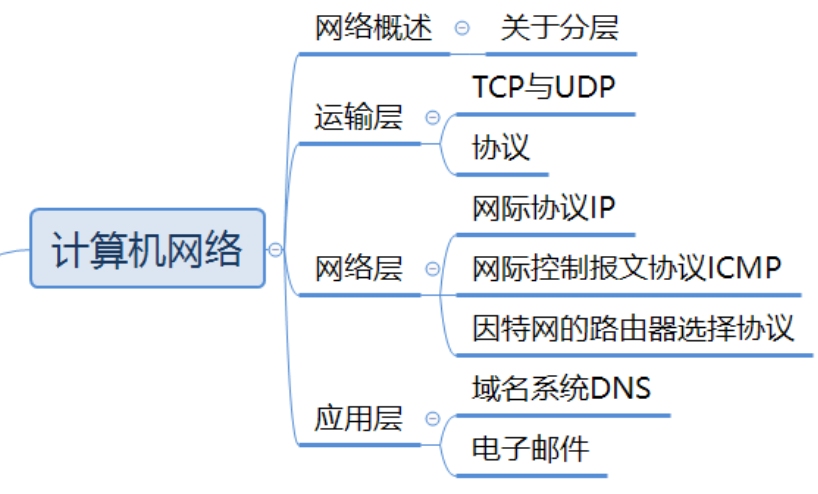
\includegraphics[width=0.85\columnwidth]{pic/overview.png}
	\caption{Overview}
	\label{fig:kernelcore}
	% \vspace{-5pt}
\end{figure}

\subsection{网络连接的方式}
\begin{enumerate}
\item 直接连接的网络(直连网)
\begin{itemize}
\item \underline{点对点(point-to-point)网络:}包括专用介质、节点/主机
\begin{itemize}
	\item 单向(simplex):如广播、电视
	\item 半双工(half duplex):异步双向,如对讲机
	\item 全双工(full duplex): 同步双向,如电话
\end{itemize}
\end{itemize}
\end{enumerate}


\section{应用层}
\section{传输层}
\section{网络层}
\section{链路层}
\end{document}
